\documentclass[11pt, oneside]{article} 
\usepackage{geometry}
\geometry{letterpaper} 
\usepackage{graphicx}
	
\usepackage{amssymb}
\usepackage{amsmath}
\usepackage{parskip}
\usepackage{color}
\usepackage{hyperref}

\graphicspath{{/Users/telliott_admin/Dropbox/Tex/png/}}
% \begin{center} 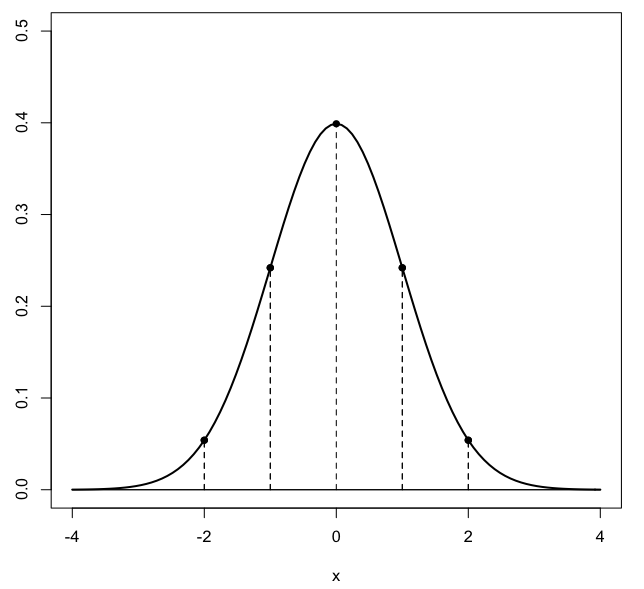
\includegraphics [scale=0.4] {gauss3.png} \end{center}

\title{More on Galois fields like $GF(2^8)$}
\date{}

\begin{document}
\maketitle
\Large

I found some other write-ups that provide a different perspective and a little more insight.

\url{http://www.cs.utsa.edu/~wagner/laws/FFM.html)}

Consider this multiplication: \textbf{ 0xb6 * 0x53}.  Write it in binary as:

\[ 1011\ 0110\ * \ 0101\ 0011 \]

We adopt a new notation.  Rewrite this as

\texttt{(7\ 5\ 4\ 2\ 1) * (6\ 4\ 1\ 0)}

This is a shorthand version of the Galois field notation:

\[ (x^7 + x^5 + x^4 + x^2 + x) * (x^6 + x^4 + x + 1) \]

The first line below restates the problem, then we do the multiplication one digit at a time.  It turns out that we can multiply by each of the digits, XOR the result, and not worry about the mod until the end.

\begin{center} 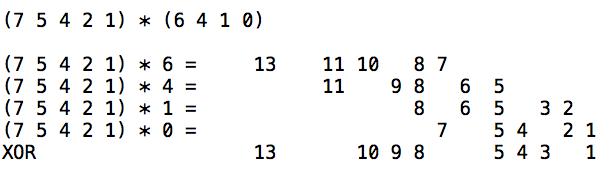
\includegraphics [scale=0.6] {GFmath1.png} \end{center}

Recall above where we said that multiplying by decimal 2, which is the same as multiplying by $x$ in the field notation, is also the same as a left-shift of 1 in the binary representation.  In the line $(7 \ 5 \ 4 \ 2 \ 1) * 6$, we simply add $6$ to each of the digits in the first number to give the result (13,11,10,8,7).  The spacing is used to simplify the XOR on the last line.

Now, we do the mod operation.
\begin{center} 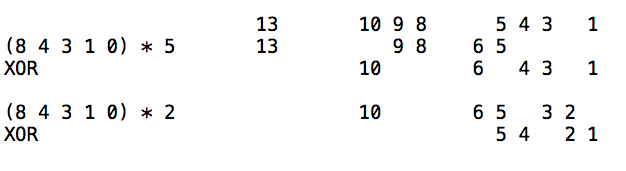
\includegraphics [scale=0.6] {GFmath2.png} \end{center}
The special divisor is $(8,4,3,1,0)$. 
\[ (x^8 + x^4 + x^3 + x + 1) \]

We multiply by $5$ to get it to align with the $13$ in the interim result.  This is the same as multiplying the irreducible polynomial by $x^5$ or multiplying its binary equivalent (1 0001 1011) by $2^5$.

After the XOR, the $13$ is gone.  We repeat the process, lining up with the $10$ and zeroing it out.  If there had been an $8$ we would go that far, but no farther.

Our answer, then, is $0011 \ 0110$ which is \textbf{0x36}.

The complete multiplication is:  \textbf{0xb6 * 0x53 = 0x36}.

Effectively what we've done is to do repeated divisions by powers of two of the super duper special number (1 0001 1011).  We guarantee that every place higher than $8$ will be turned to zero by this operation.

\subsection*{wikipedia example}

Another view of the modulus or division operation comes from the wikipedia example:  \textbf{0x53 * 0xca}.  We write this in binary:  $0101 \ 0011 \ * \ 1100 \ 1010$.

In our new notation, this would be

\begin{center} 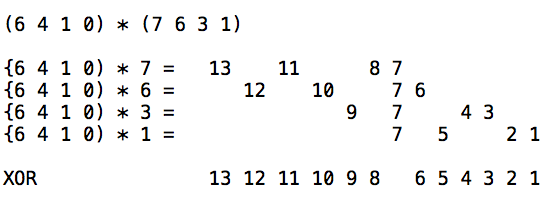
\includegraphics [scale=0.6] {GFmath3.png} \end{center}
which looks like it's pretty special.  And it is. 

 Here is the mod step:
\begin{center} 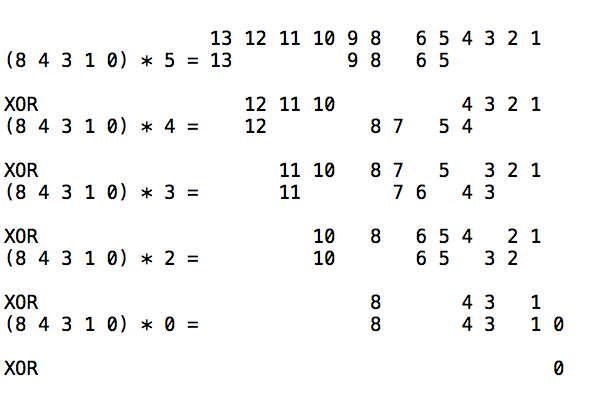
\includegraphics [scale=0.6] {GFmath4.png} \end{center}

That $0$ at the end is not really zero.  It is a power of $2$, or $2^0 =$ \textbf{0x01}.  What we've shown is that  \textbf{0x53 * 0xca = 0x01}.  In other words, \textbf{0x53} is the \emph{multiplicative inverse} of \textbf{0xca}.

Let's take a look at doing the same mod operation as long division, which should hammer  home the point we've been absorbing.
\begin{center} 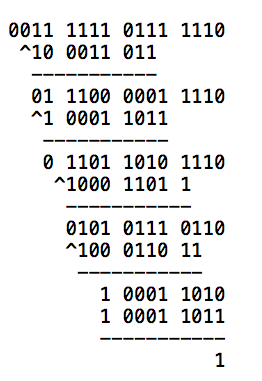
\includegraphics [scale=0.6] {GFmath5.png} \end{center}

Note, I should not have put those caret marks in this figure, they are just for alignment, and don't mean anything else.

\subsection*{extended Euclidean algorithm}
It is possible to apply the "extended" Euclidean algorithm to the problem of finding multiplicative inverses.  We developed this topic in connection with GF($2^3$).  

The calculations for GF($2^8$) are a bit hairier, but it seems to work as it should .  Here is one example:

\begin{verbatim}
100011011 is the irreducible polynomial

consider 
x^6 + x^3 + x + 1 = 1001011
we need 2 places thus q = 100
ignore the rest

a          b        q    qb
100011011  1001011  100  100101100
 
100011011
100101100
---------
   110111

a        b       q   qb
1001011  110111  11  1011001

1001011
1011001
-------
  10010

a       b      q   qb
110111  10010  11  110110
110110
------
     1

Backtrack:

110111 = 100011011 - 100 * 1001011
 10010 =   1001011 -  11 *  110111
     1 =    110111 -  11 *   10010

     1 =    110111 -  11 * [1001011 -  11 *  110111]
       = 100 * 110111 - 11 * 1001011
       = 100 [100011011 - 100 * 1001011] - 11 * 1001011
       = -10000 * 1001011 - 11 * 1001011
       = (10011) * 1001011
       = (x^4 + x + 1)(x^6 + x^3 + x + 1)

Check

(x^4 + x + 1)(x^6 + x^3 + x + 1)
= x^10 + x^7 + x^7 + x^6 + x^5 + x^4 + x^4 + x^3 + x^2 + x + x + 1
= x^10 + x^6 + x^5 + x^3 + x^2 + 1
= 100 0110 1001

mod
100 0110 1101
100 0110 11
-------------
            1
\end{verbatim}
            
We calculate that $(x^4 + x + 1)(x^6 + x^3 + x + 1) = 1$

In hex, that's \textbf{13} * \textbf{4b} = \textbf{01}.  If you check the table of multiplicative inverses, you'll see that's a match.

I don't care to do any more!

\end{document}